
\subsection{Telencephalon}
\label{subsec:Telencephalon} \index{Telencephalon}
%%%%%%%%%%%%%%%%%%%%%%%%%%%%%%%%%%%%%%%%%%%%%%%%%%%%%%%%%%%
%%%%%%%%%%%%%%%%%%%%%%%%%%%%%%%%%%%%%%%%%%%%%%%%%%%%%%%%%%%

Das Telencephalon oder das Endhirn ist eines der fünf Hirnareale, in die sich das Gehirn nach der Cephalisation gliedern lässt. Das Telencephalon befindet sich am rostralen Ende des Gehirns und überdeckt bei Säugern teilweise das superiore Diencephalon. Auch Bereiche des Mesencephalons können von ihm verdeckt werden. Generell kann das Telencephalon in cortikale Gebiete (Großhirnrinde), Mark (weiße Substanz) und subcortikale Kerngebiete, zu denen die Basalganglia und die Amygdala gehören, unterteilt werden. 

\subsubsection{Großhirnrinde}
\label{subsubsec:Grosshirnrinde}
%%%%%%%%%%%%%%%%%%%%%%%%%%%%%%%%%%%%%%%%%%%%%%%%%%%%%%%%%%%

Der cerebrale Cortex (\textit{Cortex cerebri}) \index{Cortex! cerebri} umhüllt das Gehirn und macht bei Säugern den größten Teil der Außenfläche des Gehirns aus. Er besteht aus zwei Hemisphären, die durch einen dicken Faserstrang, den \textit{Corpus callosum} \index{Corpus! callosum} oder Balken, miteinander in Verbindung stehen. Im Laufe der Evolution expandierte der cerebrale Cortex der Säuger und verdeckt dadurch jene Strukturen des Endhirns, die innerhalb der Hemisphären liegen. Im Allgemeinen dient die Großhirnrinde der Analyse und Integration sensorischer Information, sowie der Verknüpfung  dieses Inputs mit bereits gespeicherten Informationen und Erfahrungen. Des Weiteren ist der cerebrale Cortex die 'Steuerzentrale' von Verhalten, das weit über simple Reflexe und Reaktionen hinausreicht. Diese analytischen und integrativen Fähigkeiten des Cortex resultieren aus seiner zellulären Organisation, sowie aus der Kommunikation mit den restlichen Strukturen des zentralen Nervensystems \textsuperscript{\cite[Kap.~7]{watson2010thebrain}}.


\subsubsection*{Faltung der Großhirnrinde}
%%%%%%%%%%%%%%%%%%%%%%%%%%%%%%%%%%%%%%%%%%%%%%%%%%%%%%%%%%%

Basierend auf der cortikalen Faltung können Säugetiere in lissencephale und gyrencephale Spezies unterteilt werden. Die Oberfläche des Cerebralcortex der Ratte als \textbf{lissencephale Spezies}\index{lissencephal} ist eben, bzw. glatt strukturiert. Im Gegensatz dazu weist der cerebrale Cortex von \textbf{gyrencephalen Spezies}\index{gyrencephal}, wie dem Schaf oder der meisten Primaten, zahlreiche Furchen (Sulci, Fissurae) und Windungen (Gyri) auf. Die Sulci und vor allem die Fissurae reichen bis in tiefere Ebenen des Cortex und vergrößern somit dessen Gesamtoberfläche \textsuperscript{\cite[Kap.~7]{watson2010thebrain}}. Anhand dieser Fissurae und Sulci kann der cerebrale Cortex in vier Hirnlappen, \textit{Lobi cerebri}\index{Lobi cerebri}, unterteilt werden. Es kann zwischen Frontallappen, Temporallappen, Parietallappen und Okzipitallappen unterschieden werden (Abb.~\ref{fig:cortex_lappen}).\\

\noindent Die \textbf{Insula}\index{Insula}, auch Inselrinde oder \textit{Gyrus insularis}, befindet sich tief innerhalb des Sulcus lateralis und wird vom Temporal-, Parietal- und Frontallappen überdeckt. Der Bereich des cerebralen Cortex, der sie verdeckt, wird auch \textbf{Operculum} genannt. Die Insula ist an der Regulation von Emotionen und der Homoöstase beteiligt \textsuperscript{\cite[Kap.~15]{kandel2013principles}}. Des Weiteren prozessieren Neurone der Insula Informationen, die den 'inneren Zustand' des Körpers betreffen und bei autonomen Komponenten der Schmerz-Antwort mitwirken (Kap.~\ref{subsubsec:Schmerzsinn}) \textsuperscript{\cite[Kap.~24]{kandel2013principles}}. Ebenfalls ein besonderer Gyrus ist der \textbf{cinguläre Cortex}\index{Cortex! cinguli} (\textit{Gyrus cinguli}). Er umgibt die dorsale, bzw. superiore Oberfläche des Corpus callosum (Abb.~\ref{fig:schaf_lateral_sagittal}~K,L) und ist als Teilgebiet des limbischen Systems (Kap.~\ref{subsec:limisches_system}) in die Regulation von Emotionen und Kognition involviert \textsuperscript{\cite[Kap.~15]{kandel2013principles}}.

\begin{figure}[H]
	\centering
	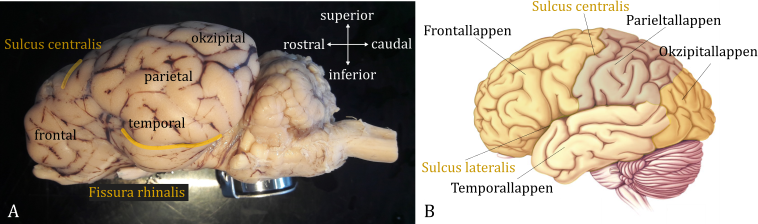
\includegraphics[width=\textwidth]{pictures/Bilder_Jule/Andere/grosshirnrinde.png}
	\caption[Lappen und Sulci der Großhirnrinde]{\textbf{Lappen und Sulci der Großhirnrinde.} \textbf{A:} Großhirnrinde des Schafes, \textbf{B:} Großhirnrinde des Menschen. Die Großhirnrinde (gelb bis bräunlich) kann anhand der Sulci in vier Lappen (\textit{Lobi cerebri}) unterteilt werden: Frontallappen, Parietallappen, Temporallappen und Okzipitallappen\index{Lobi cerebri}. \\
	Abbildung B nach \textit{Neuroanatomy}, Crossman und Neary \textsuperscript{\cite[Kap.~7]{crossman2014neuroanatomy}}.}
	\label{fig:cortex_lappen} 
\end{figure}

\noindent Die besonders großen und bedeutenden Sulci werden auch Fissuren genannt. Die wohl auffallendste unter ihnen ist die \textbf{Fissura longitudinalis cerebri}\index{Fissura! longitudinalis cerebri}. Sie befindet sich zwischen den beiden Großhirnhemisphären. Unter ihr liegt der Corpus callosum\index{Corpus! callosum}, die Hauptverbindung der beiden Hemisphären. Der \textbf{Sulcus centralis}\index{Sulcus! centralis} erstreckt sich in superior-inferiorer Richtung und trennt den Frontallappen vom Parietallappen. Der \textbf{Sulcus lateralis}\index{Sulcus! lateralis} oder auch \textit{Fissura sylvii} erstreckt sich entlang der rostro-caudalen Achse und trennt den Temporallappen vom Frontal- und Parietallappen (Abb.~\ref{fig:cortex_lappen}~B) \textsuperscript{\cite[Kap.~7]{neurowissenschaften_baer}}. Ein weiterer, bedeutender Sulcus ist die \textbf{Fissura rhinalis}\index{Fissura! rhinalis} (Abb.~\ref{fig:cortex_lappen}~A), die den Neocortex räumlich vom Archicortex trennt. 

\subsubsection*{Lappen der Großhirnrinde}
%%%%%%%%%%%%%%%%%%%%%%%%%%%%%%%%%%%%%%%%%%%%%%%%%%%%%%%%%%%

Aufgrund der Gyri und Sulci lässt sich die Großhirnrinde in vier verschiedene Lappen, die \textit{Lobi cerebri}\index{Lobi cerebri}, einteilen (Abb.~\ref{fig:cortex_lappen}). Jedem Lobus können dabei verschiedene Funktionen zugeordnet werden. Der rostral gelegene \textbf{Frontallappen} ist am Kurzzeitgedächtnis, der Planung zukünftiger Handlungen, sowie an der Steuerung der Motorik beteiligt. Der laterale \textbf{Temporallappen} kann mit dem Hören assoziiert werden. Zudem ist er durch die tiefer gelegenen Strukturen des Hippocampus und der Amygdala an Lernvorgängen, Gedächtnisbildung und der Entstehung von Emotionen beteiligt. Der \textbf{Parietallappen} ist caudal hinter dem Frontallappen und superior des Temporallappens lokalisiert. In ihm wird die somatosensorische Wahrnehmung prozessiert. Dabei entsteht ein Eindruck des eigenen Körpers relativ zur räumlichen Umgebung. Der vierte Lobus ist der \textbf{Okzipitallappen}, der sich am caudalen Ende der Großhirnrinde befindet. Er enthält die primären und auch höheren visuellen Areale \textsuperscript{\cite[Kap.~1]{kandel2013principles}}.

\subsubsection*{Sensorische und Motorische Felder}
\label{subsubsec:Sens_Mot_Felder}
%%%%%%%%%%%%%%%%%%%%%%%%%%%%%%%%%%%%%%%%%%%%%%%%%%%%%%%%%%%

\index{Sensorik! allgemein}
In der Großhirnrinde findet die Informationsverarbeitung in verschiedenen Arealen statt. Sie lässt sich funktionell in \textbf{primär motorische}\index{Motorik! allgemein} und \textbf{primär sensorische Felder} unterteilen. Der primäre Motorcortex (M1) enthält Neurone, die an den $\upalpha$-Motorneuronen im Ventralhorn des Rückenmarks enden. Er ist rostral des \textit{Sulcus centralis}\index{Sulcus! centralis}, auf dem \textit{Gyrus praecentralis}\index{Sulcus! praecentralis}, lokalisiert. Zu den primären sensorischen Feldern gehören der primäre visuelle Cortex (V1) am caudalen Ende des Okzipitallappens, der primäre auditorische Cortex (A1) im Temporallappen, sowie der primäre somatosensorische Cortex (S1) caudal des \textit{Sulcus centralis} auf dem \textit{Gyrus postcentralis}. Alle drei primären sensorischen Felder erhalten hauptsächlich unimodale Information aus den zugehörigen thalamischen Kernen. Dabei ist jedes Sinnesorgan, also Augen, Ohren und die Haut, mehrfach im zugehörigen sensorischen Feld repräsentiert. Diese Repräsentation zeigt dabei eine retinotope, tonotope, bzw. somatotope Organisation. Die \textbf{Topologie}, also die Lagebeziehung, der abgebildeten Information bleibt dabei bestehen. Das Größenverhältnis einzelner Teilgebiete wird jedoch nicht zwingend beibehalten \textsuperscript{\cite[Kap.~14]{penzlin2005tierphys}}. Oft findet eine \textbf{Überrepräsentation} verhaltensrelevanter Bereiche in den primären sensorischen oder motorischen Cortices statt. Beispielsweise werden bei Säugern der retinale Bereich der Fovea im V1 \textsuperscript{\cite{overrepresentation_fovea}}, sowie einige Bereiche der Körperoberfläche in S1 und M1 \textsuperscript{\cite[Kap.~14]{penzlin2005tierphys}}, überrepräsentiert. Die \textbf{sekundären}, \textbf{tertiären}, usw. \textbf{Repräsentationsfelder} sind den primären untergeordnet. Die sekundären Felder erhalten spezifische thalamische Projektionen.\\

\begin{figure}[H]
    \centering
    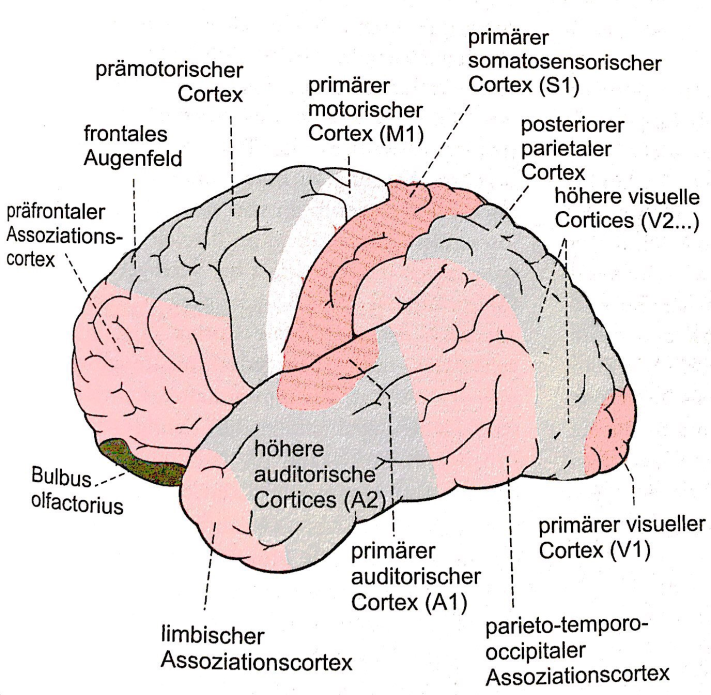
\includegraphics[width=0.69\textwidth]{pictures/Bilder_Jule/Andere/Grosshirnrinde_sensorik_motorik.png}
    \caption[Sensorische, motorische und assoziative Areale der Großhirnrinde]{\textbf{Sensorische, motorische und assoziative Areale der Großhirnrinde.} Abbildung aus \textit{Lehrbuch der Tierphysiologie}, Pezlin \textsuperscript{\cite[Kap.~14]{penzlin2005tierphys}}.}
    \label{fig:grosshirnrinde_sensorik_motorik}
\end{figure}

\noindent Jene Felder, die weder den sensorischen noch den motorischen Feldern zugeordnet werden können, werden als sogenannter unspezifischer oder \textbf{assoziativer Cortex} bezeichnet. In diesen Arealen findet eine Verknüpfung oder Integration von motorischer und multisensorischer Information statt \textsuperscript{\cite[Kap.~14]{penzlin2005tierphys}}. 

\noindent Die Ausdehnung der Projektionsfelder, sowie das Verhältnis zwischen den motorischen und sensorischen Feldern und den Assoziationsfeldern, variiert zwischen den verschiedenen Tierklassen. Zum einen nimmt der Anteil der assoziativen, unspezifischen Felder mit der Höherentwicklung zu \textsuperscript{\cite[Kap.~14]{penzlin2005tierphys}}. Zum anderen sind Felder, die für die Lebensweise einer Tierart besonders relevant sind, wie zum Beispiel das olfaktorische Feld bei Ratten, vergrößert (Abb.~\ref{fig:grosshinrinde_vgl}).

\begin{figure}[H]
    \centering
    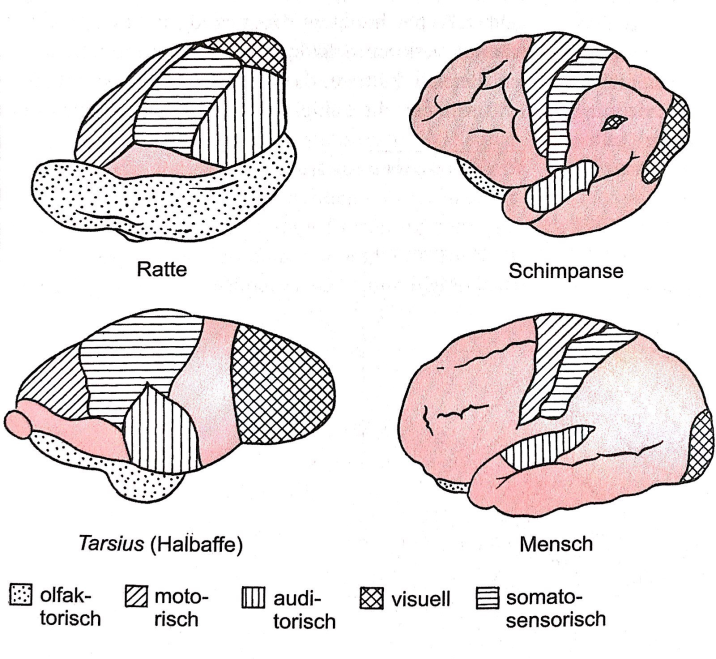
\includegraphics[width=0.7\textwidth]{pictures/Bilder_Jule/Andere/grosshirnrinde_vgl.png}
    \caption[Verhältnis sensorischer, motorischer und assoziativer Areale der Großhirnrinde]{\textbf{Verhältnis sensorischer, motorischer und assoziativer Areale der Großhirnrinde.} Dargestellt ist die Ausdehnung der sensorischen und motorischen Projektionsfelder (schwarz-weiß) und der assoziativen Felder (rot) verschiedener Säugetiere. Abbildung aus \textit{Lehrbuch der Tierphysiologie}, Penzlin \textsuperscript{\cite[Kap.~14]{penzlin2005tierphys}}.}
    \label{fig:grosshinrinde_vgl}
\end{figure}{}

\subsubsection*{Der Neocortex} \index {Neocortex}
%%%%%%%%%%%%%%%%%%%%%%%%%%%%%%%%%%%%%%%%%%%%%%%%%%%%%%%%%%%

In evolutionär älteren Arealen des Cortex, wie dem olfaktorischen Cortex, besteht die Großhirnrinde aus nur drei Schichten, während der evolutionär jüngere \textbf{Neocortex}, auch Isocortex, aus sechs Schichten aufgebaut ist. Obwohl sich die verschiedenen Areale des Neocortex funktionell unterscheiden und beispielsweise Informationen unterschiedlicher sensorischer Systeme verarbeiten, variiert lediglich die Dicke der Zellschichten, jedoch nicht ihre Anzahl und Reihenfolge. Diese zellulären Schichten bilden die sogenannte \textbf{graue Substanz}\index{graue Substanz} des (Neo-)Cortex, die viele Zellkörper, jedoch wenige Fasern enthält. Diese Schichten werden von Außen nach Innen nummeriert und bestehen aus drei prominenten Zelltypen: exzitatorische Pyramidenzellen, Körnerzellen, zu denen auch die bedornten Sternzellen (\textit{spiny stellate cells}) gehören, und inhibitorische Interneurone. Jede der sechs Zellschichten des Neocortex besitzt charakteristische Zellen und  Verknüpfungen (Abb.~\ref{fig:neoccortex_schichtung}) \textsuperscript{\cite[Kap.~7]{watson2010thebrain}}. 

\begin{figure}[H]
	\centering
	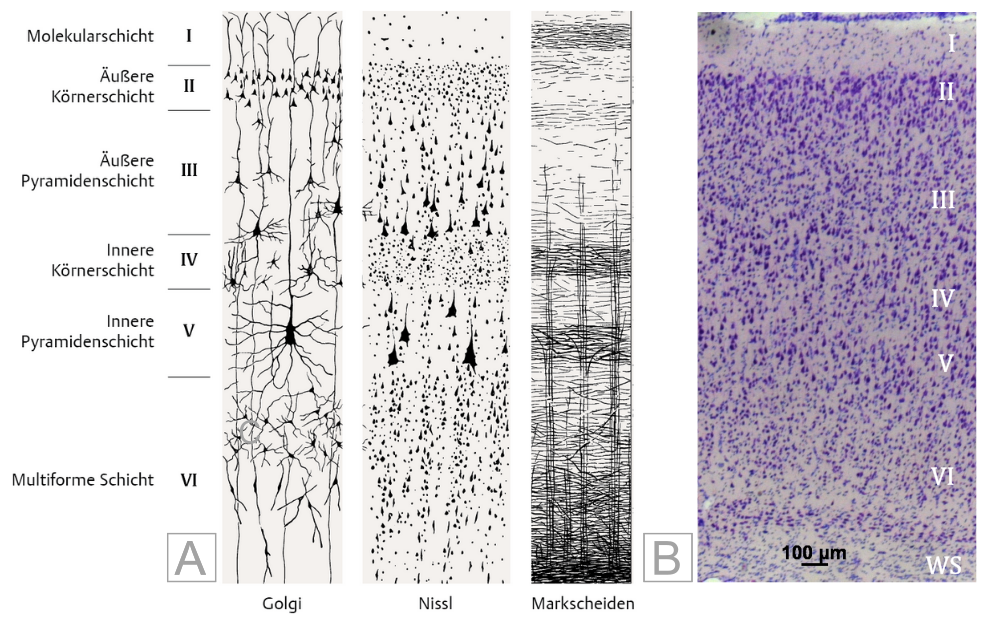
\includegraphics[width=\textwidth]{pictures/Bilder_Jule/Andere/neocortex_schichtung.png}
	\caption[Schichtung des Neocortex]{\textbf{Schichtung des Neocortex.} \textbf{A}:~Schematische Darstellung der Schichten des Neocortex des Menschen unter Verwendung der Golgi-, Nissl- und Markscheidenfärbung. \textbf{B}:~Mikroskopie des Neocortex der Ratte unter Verwendung der Nisslfärbung. WS = weiße Substanz - darüber die sechsschichtige graue Substanz.\\
	Abbildung A aus \textit{Taschenlehrbuch Histologie}, Lüllmann-Rauch und Asan \textsuperscript{\cite{taschenbuch_histologie}}.}
	\label{fig:neoccortex_schichtung}
\end{figure}

\noindent Die \textbf{Molekularschicht} stellt die äußerste Schicht dar. Diese dünne Faserschicht beinhaltet nur wenige Zellkörper, jedoch viele dendritische Fortsätze und stellt somit eine Verarbeitungsstruktur des Cortex dar. Unter ihr liegt die \textbf{äußere Körnerschicht}. Sie besteht aus zahlreichen kleinen Pyramidenzellen, sowie kleinen inhibitorischen Zellen. Diese agieren in kleinen neuronalen Schaltkreisen um einkommende Information zu prozessieren. Die dritte Zellschicht, die \textbf{äußere Pyramidenschicht}, zeichnet sich durch eine Vielzahl größerer Pyramidenzellen aus. Diese senden exzitatorische Signale in benachbarte oder auch weit entfernte Areale des Cortex. Korbzellen (\textit{basket cells})  und andere inhibitorische Zellen inhibieren benachbarte Zellen und ermöglichen somit weitere cortikale Informationsverarbeitung. In der vierten Schicht, der \textbf{inneren Körnerschicht}, enden viele thalamische Fasern. Sie besteht aus zahlreichen kleinen Sternzellen. Unter ihr liegt die \textbf{innere Pyramidenschicht}, die aus den größten Pyramidenzellen des Neocortex aufgebaut ist. Ihre Axone, die bis weit außerhalb des Neocortex reichen, terminieren unter anderem im Striatum und Rückenmark. Die am tiefsten gelegene Schicht ist die sechste, \textbf{multiforme Schicht}. Diese Schicht ist aus vielen kleinen Zellen aufgebaut, unter anderem aus kleinen Pyramidenzellen, die in den Thalamus projizieren. Diese Verbindungen schließen die Rückkopplungsschleife zwischen Cortex und Thalamus, die die thalamische Aktivität reguliert \textsuperscript{\cite[Kap.~7]{watson2010thebrain}}.\\
Die neuronalen Netzwerke, die die cortikale Informationsverarbeitung dominieren, zeigen Aktivität, die \textbf{in Säulen organisiert} ist: Die Zellen des Neocortex zeigen die meisten Verbindungen zu Zellen oberhalb und unterhalb der eigenen Position. Dabei weisen einige Zellen inhibitorische Verbindungen zu benachbarten Säulen auf. Diese Verschaltungen scheinen die cortikale Aktivität zu fokussieren.\\
\noindent Unterhalb der neocortikalen Schichten liegt die sog. \textbf{weiße Substanz}\index{weiße Substanz} - eine dichte Schicht aus axonalen Fasern, die nur wenige Zellkörper beinhaltet. Diese Fasern ermöglichen die Verbindung und Kommunikation verschiedener Areale des Cortex, sowie die Kommunikation mit dem Rest des Nervensystems \textsuperscript{\cite[Kap.~7]{watson2010thebrain}}.

\subsubsection*{Der Allocortex} \index{Allocortex}
%%%%%%%%%%%%%%%%%%%%%%%%%%%%%%%%%%%%%%%%%%%%%%%%%%%%%%%%%%%

Der sogenannte Allocortex setzt sich aus dem Archicortex und dem Paleocortex zusammen und ist, genau wie der Neocortex, Teil der Großhirnrinde. Der mediale \textbf{Archicortex}\index{Archicortex} der Säugetiere ist aus drei Zellschichten aufgebaut und wird auch Hippocampusregion genannt. Die \textbf{Fissura rhinalis} trennt den evolutionär älteren Archicortex vom jüngeren, sechsschichtigen Neocortex (Abb.~\ref{fig:allocortex_ratte}) \textsuperscript{\cite[Kap.~6]{storch2012lehrbuchzoo}}. Neben dem Hippocampus ist auch der cinguläre Cortex\index{Cortex! cinguli} (Kap.~\ref{subsubsec:Grosshirnrinde}, Kap.~\ref{subsec:limisches_system}) ein Teilgebiet des Archicortex. Der lateral gelegene \textbf{Paleocortex}\index{Paleocortex} ist das älteste Teilgebiet der Großhirnrinde. Genau wie der Archicortex besteht er aus drei Zellschichten \textsuperscript{\cite[Kap.~6]{storch2012lehrbuchzoo}}. Er bildet bei Säugern das Riechhirn und beinhaltet den primären olfaktorischen Cortex, den Bulbus olfactorius\index{Bulbus olfactorius}, sowie die cortikalen Bereiche der Amygdala\index{Amygdala} \textsuperscript{\cite[Kap.~9]{trepel2011neuroanatomie}}.

\begin{figure}[H]
    \centering
    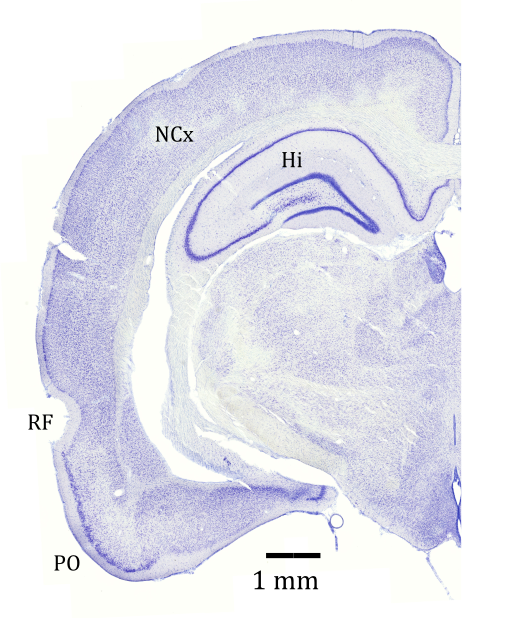
\includegraphics[width=0.38\textwidth]{pictures/Bilder_Jule/Ratte/RF.png}
    \caption[Großhirnrinde Ratte]{\textbf{Großhirnrinde Ratte.} Coronaler Querschnitt durch eine Hemisphäre des Rattengehirns (N21-3). Der dreischichtige Hippocampus (Hi) ist Teil des Archicortex, der dreischichtige primäre olfaktorische Cortex (PO) gehört zum Paleocortex. Die Fissura rhinalis (RF) trennt den sechsschichtigen Neocortex (NCx) vom Paleocortex.}
    \label{fig:allocortex_ratte}
\end{figure}{}

\subsubsection*{Hippocampus}
\label{subsubsec:Hippocampus} \index{Hippocampus}
%%%%%%%%%%%%%%%%%%%%%%%%%%%%%%%%%%%%%%%%%%%%%%%%%%%%%%%%%%%

Das Wort 'Hippocampus' kommt aus dem Griechischen und bedeutet Seepferdchen. Der Hippocampus ist Teil des Archicortex und folglich aus drei Zellschichten aufgebaut. Sowohl bei Menschen, als auch bei der Ratte zeichnet sich der Hippocampus durch eine c-förmige Struktur aus \textsuperscript{\cite[Kap.~20]{paxinos2014rat}}, die den Thalamus umgibt (Abb.~\ref{fig:hippocampus_schaf}). Er hängt dabei am inneren Rand der Großhirnrinde und liegt zum Großteil an den medialen Wänden der lateralen Ventrikel. Caudal reicht der Hippocampus bis vor zur Vierhügelplatte. Superior reicht er bis an den \textit{Corpus callosum}, wo er unterhalb des Balkens in die Faserstruktur des \textbf{Fornix}\index{Fornix} übergeht, der bis in den \textbf{Mammillarkörper} zieht. Die \textbf{Fimbria}\index{Fimbria} enthält afferente und efferente Fasern und geht in den Fornix über \textsuperscript{\cite[Kap.~9]{trepel2011neuroanatomie}}.\\

\begin{figure}[H]
    \centering
    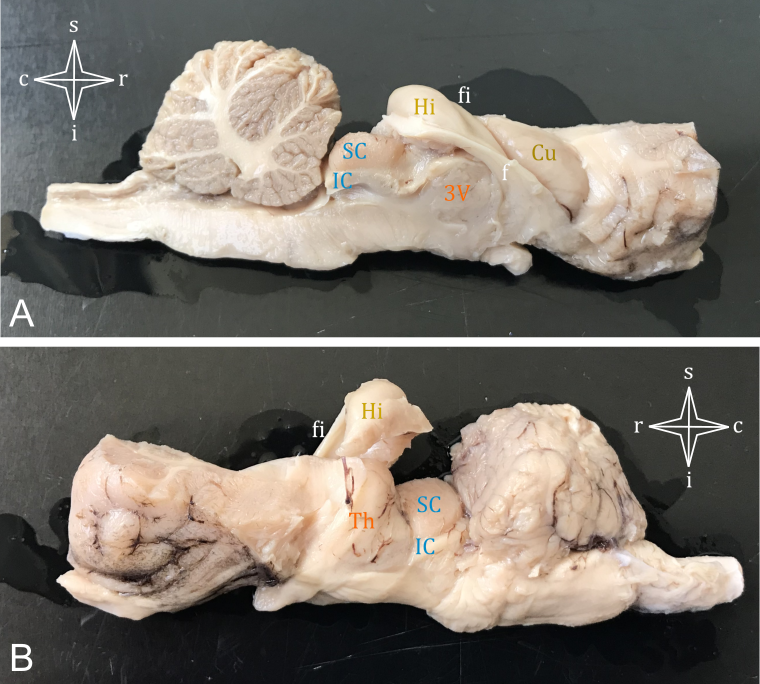
\includegraphics[width=0.6\textwidth]{pictures/Bilder_Jule/Schaf/Ausschnitte/hippocampus_schaf.png}
    \caption[Hippocampus Schaf]{\textbf{Hippocampus Schaf.} Gezeigt ist das Ergebnis einer Hippocampus-Präparation am Schafshirn. Dabei wurden die Bereiche der Großhirnrinde, die den Hippocampus verdecken, entfernt. Zu sehen sind der Hippocampus (Hi), der den Thalamus (Th) umschließt. Er liegt caudal des Nucleus caudatus (Cu) und rostral der Vierhügelplatte, die aus dem Colliculus superior (SC) und dem Colliculus inferior (IC) besteht. Ebenfalls gekennzeichnet sind die Fimbria (fi), die in den Fornix (f) übergeht, sowie der dritte Ventrikel (3V), dessen Wände in Teilen vom Thalamus gebildet werden.}
    \label{fig:hippocampus_schaf}
\end{figure}{}

\noindent Die afferenten Fasern, die den Hippocampus erreichen, stammen unter anderem aus dem Neocortex und den olfaktorischen Arealen der Großhirnrinde. Über den Fornix erhält er zusätzlich Informationen aus dem Thalamus, dem cingulären Cortex (\textit{Corpus cinguli}) und der Amygdala. Im Fornix\index{Fornix} verlaufen zudem nahezu alle Efferenzen des Hippocampus. Diese enden unter anderem im Septum, in der Amygdala, sowie im Hypothalamus. Der Großteil der Fasern endet jedoch im Mammillarkörper \textsuperscript{\cite[Kap.~9]{trepel2011neuroanatomie}}.\\

\noindent Als wichtiger Bestandteil des limbischen Systems (Kap.~\ref{subsec:limisches_system}) ist der Hippocampus an emotionalen, endokrinen und vegetativen Vorgängen beteiligt \textsuperscript{\cite[Kap.~9]{trepel2011neuroanatomie}}. Des Weiteren spielt er eine wichtige Rolle in der Gedächtnisbildung. So ist der Hippocampus beispielsweise für den Transfer von gespeicherter Information vom Kurzzeit- ins Langzeitgedächtnis unabdingbar \textsuperscript{\cite[Kap.~6]{storch2012lehrbuchzoo}}. Durch synaptische Langzeit-Plastizität wird Information zeitweise im Hippocampus gespeichert. Schließlich werden die Informationen in den Neocortex, den Ort des Langzeitgedächtnisses, transferiert \textsuperscript{\cite[Kap.~18]{kandel2013principles}}.

\begin{figure}[H]
    \centering
    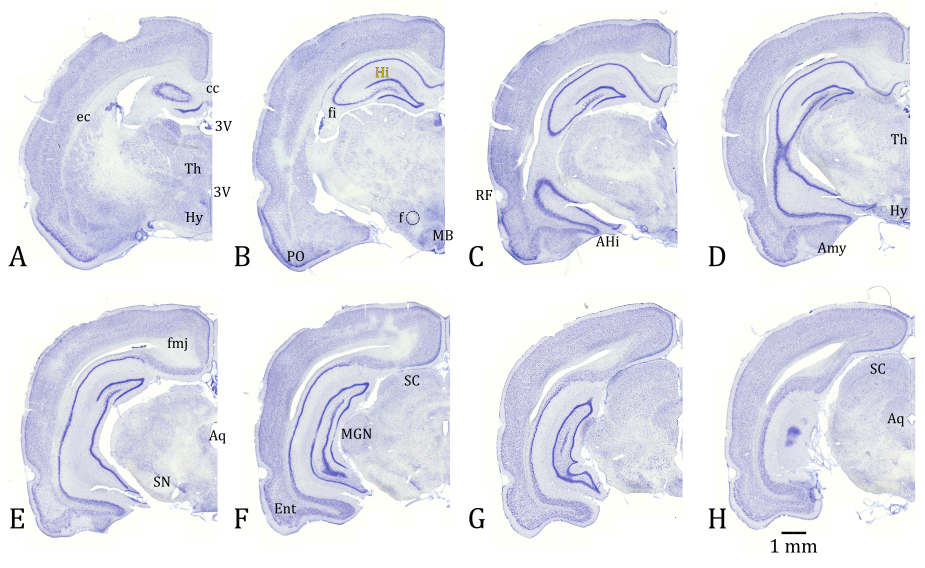
\includegraphics[width=\textwidth]{pictures/Bilder_Jule/Ratte/hippocampus.png}
    \caption[Hippocampus Ratte]{\textbf{Hippocampus Ratte.} Coronalschnitte von rostral nach caudal (A-H: N25-1, N22-2, N20-4, N20-1, N19-1, N18-1, N17-1, N16-1). Gekennzeichnet sind der Hippocampus (Hi), der den Thalamus (Th) umgibt, sowie die Fimbria (fi) und der Fornix (f). Ebenfalls gekennzeichnete Strukturen des Telencephalons: Capsula externa (ec), Corpus callosum (cc), Forceps minor des cc (fmj), Fissura rhinalis (RF), entorhinaler Cortex  (Ent), primärer olfaktorischer Cortex (PO), amygdalo-hippocampisches Areal (AHi), Amygdala (Amy). Strukturen des Diencephalons: dritter Ventrikel (3V), Hypothalamus (Hy), Mammillarkörper (MB), Corpus geniculatum mediale (MGN). Strukturen des Mesencephalons: Aquädukt (Aq), Colliculus superior (SC), Substantia nigra (SN).}
    \label{fig:hippocampus_ratte}
\end{figure}{}

\subsubsection*{Cortico-cortikale Verbindungen}
\label{subsubsec:cortico-cortical}
%%%%%%%%%%%%%%%%%%%%%%%%%%%%%%%%%%%%%%%%%%%%%%%%%%%%%%%%%

Die weiße Substanz, die unter der Oberfläche des Cortex liegt, kann nach ihrem Ursprung, bzw. ihrer Termination, in drei verschiedene Klassen unterteilt werden: Assoziationsfasern, Kommissuren und Projektionsfasern.
\textbf{Assoziationsfasern} verbinden cortikale Areale, die innerhalb derselben Großhirnhemisphäre liegen. Dabei kann zwischen langen und kurzen Fasern unterschieden werden. Durch die kurzen Assoziationsfasern stehen benachbarte cortikale Sulci miteinander in Verbindung. Die langen Fasern ermöglichen eine Interaktion weit entfernter Areale. So sind über die langen Assoziationsfasern die primären sensorischen Areale mit den Assoziationsarealen des Cortex verbunden. Der \textit{Fasciculus longitudinalis inferior}\index{Fasciculus! longitudinalis} (Abb.~\ref{fig:cortico-cortical}) beispielsweise verbindet den Frontal- mit dem Okzipitallappen. Eine seiner Teilgebiete, der \textit{Fasciculus arcuatus}\index{Fasciculus! arcuatus}, vernetzt Gyri des Frontal- und Temporallappens und ist essentiell für die Sprachfunktion. Der \textit{Fasciculus longitudinalis superior}\index{Fasciculus! longitudinalis} verläuft ausgehend vom Okzipitallappen bis hin zum Pol des Temporallappens und trägt so zur visuellen Wiedererkennung bei. Der \textit{Fasciculus uncinatus}\index{Fasciculus! uncinatus} verbindet anteriore und inferiore Bereiche des Frontallappens mit dem Temporallappen. Diese Projektion spielt eine wichtige Rolle in der Regulation von Verhalten. Das \textit{Cingulum}\index{Cingulum} ist im cingulären Cortex (Kap.~\ref{subsubsec:Grosshirnrinde}) lokalisiert. Durch das Cingulum stehen Frontal- und Parietallappen mit dem Gyrus parahippocampalis und angrenzenden temporalen Gyri in Verbindung.

\begin{figure}[H]
    \centering
    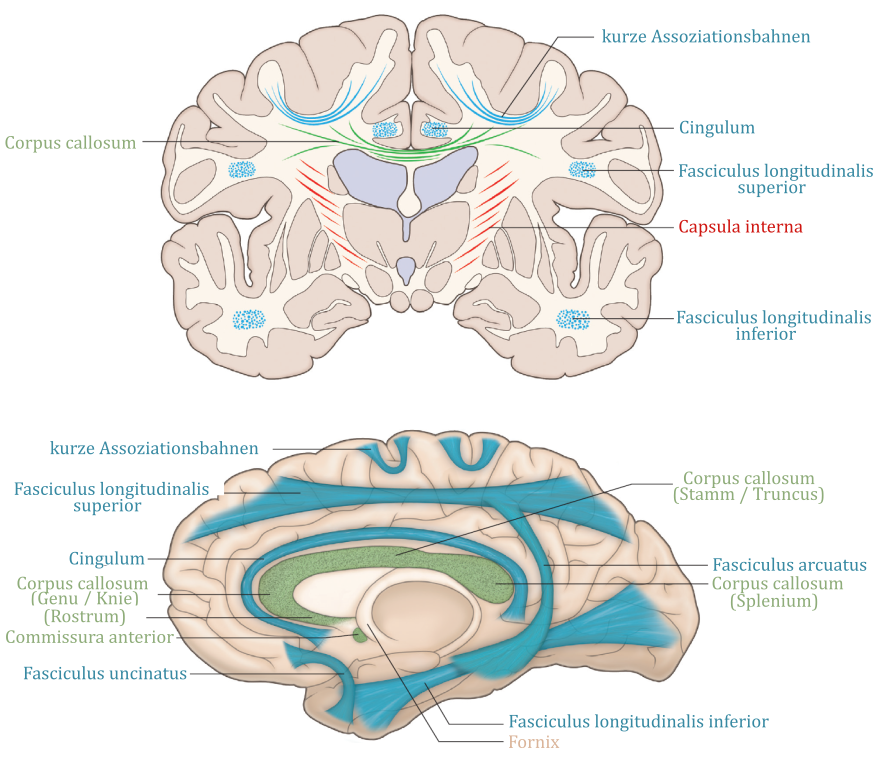
\includegraphics[width=\textwidth]{pictures/Bilder_Jule/Andere/cortico-cortical_(crossm13).png}
    \caption[Cortico-cortikale Verbindungen]{\textbf{Cortico-cortikale Verbindungen.} Verlauf der neuronalen Bahnen des cerebralen Cortex in der Coronal-Ebene (oben) und Midsagittal-Ebene (unten).\\
    Abbildung nach \textit{Neuroanatomy}, Crossman und Neary \textsuperscript{\cite[Kap.~13]{crossman2014neuroanatomy}}.}
    \label{fig:cortico-cortical}
\end{figure}{}

\noindent \textbf{Kommissuren} (Abb.~\ref{fig:faser_cortico-cortical}) verlaufen von einer Großhirnhemisphäre in die jeweils andere und verbinden somit funktionell verwandte Strukturen. Die wohl auffälligste Kommissur ist der \textit{Corpus callosum}\index{Corpus! callosum}, der zwischen den beiden Großhirnhemisphären verläuft. Er verbindet Bereiche des Neocortex, mit Ausnahme der temporalen Bereiche. Auch das \textit{Splenium} des Corpus callosum gehört zu den Kommissuren. Es verbindet die Okzipitallappen miteinander und trägt so zu visuellen Funktionen bei. Die inferioren und medialen Gyri des Temporallappens, sowie die olfaktorischen Gebiete der beiden Hemisphären, sind über die \textit{Commissura anterior} vernetzt. Den letzten Faser-Typ stellen die sogenannten \textbf{Projektionsfasern} dar. Über diese kommuniziert der cerebrale Cortex mit subcortikalen Strukturen, sowie dem Thalamus, dem Striatum, dem Hirnstamm und dem Rückenmark. Die \textit{Capsula interna}\index{Capsula interna} liegt  medial zwischen Thalamus und Nucleus caudatus. Sie kann in verschiedene Teilgebiete differenziert werden und verbindet unter anderem Thalamus und Präfrontallappen, sowie den Thalamus mit dem primären somatosensorischen, auditorischen und visuellen Cortex \textsuperscript{\cite[Kap.~13]{crossman2014neuroanatomy}}.

\begin{figure}[H]
    \centering
    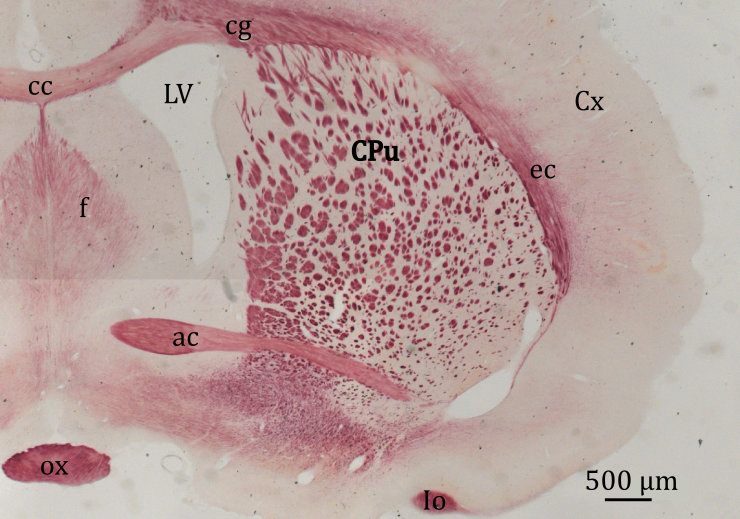
\includegraphics[width=0.45\textwidth]{pictures/Bilder_Jule/Ratte/faser_cortex.png}
    \caption[Kommissuren der Großhirnrinde]{\textbf{Kommissuren der Großhirnrinde.} Coronalschnitt durch das Rattengehirn auf Höhe des Diencephalons (F27-4). Die Commissura anterior (ac), sowie der Corpus callosum (cc) und das Cingulum (cg) sind gekennzeichnet. Ebenfalls sichtbar sind das Chiasma opticum (ox) des Diencephalons und der Fornix (f). Auch der laterale Ventrikel des Telencephalons (LV), der cerebrale Cortex (Cx), das Caudoputamen (CPu), die Capsula externa (ec) und der laterale olfaktorische Trakt (lo) sind zu sehen.}
    \label{fig:faser_cortico-cortical}
\end{figure}

\subsubsection{Amygdala}
\label{subsubsec:Amygdala} \index{Amygdala}
%%%%%%%%%%%%%%%%%%%%%%%%%%%%%%%%%%%%%%%%%%%%%%%%%%%%%%%%%%%

Die Amygdala (\textit{Corpus amygdaloideum}), auch Mandelkern genannt, liegt unterhalb des olfaktorischen Cortex und rostral des Hippocampus (Abb.~\ref{fig:amygdala_ratte}). Sie ist ein subcortikales Gebiet, das in Teilen dem Paleocortex zuzuordnen ist \textsuperscript{\cite[Kap.~9]{trepel2011neuroanatomie}}. Die Amygdala ist, wie auch der Hippocampus, ein wichtiger Bestandteil des limbischen Systems (Kap.~\ref{subsec:limisches_system}) \textsuperscript{\cite[Kap.~15]{kandel2013principles}}.

\begin{figure}[H]
    \centering
    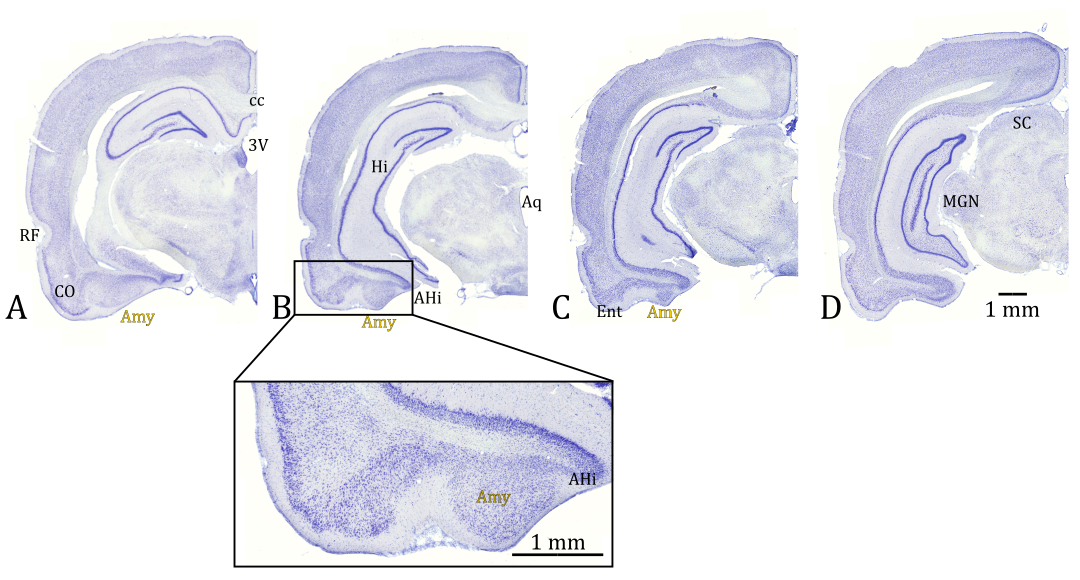
\includegraphics[width=\textwidth]{pictures/Bilder_Jule/Ratte/amygdala.png}
    \caption[Amygdala Ratte]{\textbf{Amygdala Ratte.} Coronalschnitte von rostral nach caudal (A-D: N20-2, N19-3, N18-4, N17-3). Die Amygdala (Amy) liegt unter dem olfaktorischen Cortex (CO). Das amygdalo-hippocampische Areal (AHi) stellt den Übergang zwischen der Amygdala und dem Hippocampus (Hi) dar. Ebenfalls gekennzeichnet sind der Corpus callosum (cc) und die Fissura rhinalis (RF) des Telencephalons, der Corpus geniculatum mediale (MGN) und der dritte Ventrikel (3V) des Diencephalons, sowie das Aquädukt (Aq) und der Colliculus superior (SC) des Mesencephalons.}
    \label{fig:amygdala_ratte}
\end{figure}{}

\noindent Die Amygdala besteht aus mehreren Kernen, die sich in drei Unterbereiche gliedern lassen: Der Zentralbereich steuert vegetative und affektive Grundfunktionen. Der cortico-mediale Bereich verarbeitet olfaktorische Informationen, wie zum Beispiel soziale Gerüche (Pheromone). Der dritte, baso-laterale Teilbereich ist mit Emotionen assoziiert \textsuperscript{\cite[Kap.~6]{storch2012lehrbuchzoo}}. Im Allgemeinen ist die Amygdala in die Entstehung und Verarbeitung emotionaler Zustände, wie der Angst- und   Vermeidungsreaktion, involviert. Sie spielt auch bei positiven Emotionen, besonders wenn das Belohnungssystem involviert ist, eine Rolle \textsuperscript{\cite[Kap.~48]{kandel2013principles}}.\\
Die Amygdala erhält direkten und indirekten thalamischen Input. Somit ist sie in der Lage die emotionale Ladung eines Stimulus zu evaluieren. Detektiert sie Gefahr, kann sie durch ihre starke  Verbindung zu Hypothalamus und Hirnstamm die Entstehung von physiologischen und endokrinen Antworten und Verhaltensreaktionen dirigieren \textsuperscript{\cite[Kap.~48]{kandel2013principles}}. Zum Beispiel kann die Amygdala unbewusste Reaktionen auf Angstzustände, wie die Veränderung von Puls, Respirationsrate und Pupillen-Erweiterung,  hervorrufen \textsuperscript{\cite[Kap.~15]{kandel2013principles}}.
Auch instinktive Prozesse, wie Hunger oder Durst, sowie Prozesse, die Angst-, Aggressions- oder Paarungsverhalten untergeordnet sind, werden von der Amygdala gesteuert \textsuperscript{\cite[Kap.~18]{kandel2013principles}}.
Die vielseitigen Projektionen, die von der Amygdala ausgehen, erlauben ihr auch andere, kognitive Funktionen zu beeinflussen. Beispielsweise können durch die Amygdala mittels umfassender Projektionen in cortikale Gebiete sowohl Aufmerksamkeit als auch Wahrnehmung, Gedächtnis und Entscheidungsfindung moduliert und somit beeinflusst werden. Durch ihre Verbindung mit den modulatorischen Nuclei, wie Teilen der dopaminergen, noradrenergen und serotonergen Systeme (Kap.~\ref{sec:transmittersysteme}), ist sie zudem in der Lage die kognitive Sachverarbeitung zu beeinflussen \textsuperscript{\cite[Kap.~48]{kandel2013principles}}.

\subsubsection{Basalganglia}
\label{subsec:Basalganglia} \index{Basalganglia}
%%%%%%%%%%%%%%%%%%%%%%%%%%%%%%%%%%%%%%%%%%%%%%%%%%%%%%%%%%%
%%%%%%%%%%%%%%%%%%%%%%%%%%%%%%%%%%%%%%%%%%%%%%%%%%%%%%%%%%%

Der Begriff der Basalganglia (Kap.~\ref{subsec:basalganglien}) umschreibt Bestandteile des Tel-, Di- und Mes-

\begin{wrapfigure}{r}{0.42\textwidth}
    \centering
    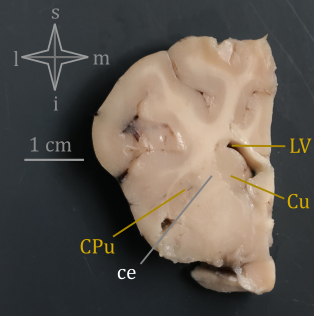
\includegraphics[width=0.42\textwidth]{pictures/Bilder_Jule/Schaf/Ausschnitte/Striatum.png}
    \caption[Striatum Schaf]{\textbf{Striatum Schaf.} Das Striatum des Schafes besteht aus dem Nucleus caudatus (Cu) und dem Putamen (CPu), die von der Capsula externa (ce), die aus vielen Fasern besteht, voneinander getrennt werden. Der Nucleus caudatus bildet die laterale Seitenwand des lateralen Ventrikels (LV).}
    \label{fig:striatum}
\end{wrapfigure}

\noindent encephalons. Einen Großteil der Basalganglia besteht aus dem telencephalen \textbf{Striatum}, das bei Säugern in \textbf{Putamen} und \textbf{Nucleus caudatus} \index{Nucleus! caudatus} unterteilt werden kann. Der Nucleus caudatus legt sich c-förmig um das Putamen, das eine platte Scheibe bildet, und folgt dabei der Oberfläche des lateralen Ventrikels, dessen Seitenwand er bildet. Vor dem Ende des Nucleus caudatus liegt die Amygdala. Auch das diencephale \textbf{Pallidum}, \textit{Globus pallidus}, gehört zu den Basalganglia. Durch die Capsula interna werden Putamen und Pallidum vom Thalamus getrennt (Abb.~\ref{fig:striatum}). Die Capsula interna verläuft auch zwischen dem Putamen und dem Nucleus caudatus. Die einzelnen Bestandteile der Basalganglia erhalten ihre Afferenzen unter anderem aus dem Cortex und den anderen Subbereichen der Basalganglia. Die Efferenzen verlaufen über den Thalamus. Funktionell können den Basalganglia neben den 'klassischen Bestandteilen' auch der \textbf{Nucleus subthalamus} (Diencephalon) und die \textbf{Substantia nigra} (Mesencephalon) zugeordnet werden.
Im Allgemeinen besteht die Funktion der Basalganglia in der Regulation der Motorik \textsuperscript{\cite[Kap.~9]{trepel2011neuroanatomie}}.


